\subsection*{Άσκηση 7}

Έστω απλό $\lambda$-πλευρικά συνεκτικό γράφημα $G$ με $n$ κορυφές και ελάχιστο βαθμό κορυφής $\delta(G)$.  
\begin{enumerate}[(i)]
\item
Δείξτε ότι αν $\delta(G) \ge n/2$ τότε $\lambda = \delta(G)$.
\item
Βρείτε απλό γράφημα $G$ με $\delta(G)=\lfloor n/2\rfloor - 1$ και $\lambda < \delta(G)$.
\end{enumerate}

\subsubsection*{Λύση}

\begin{enumerate}[(i)]
\item
Καταρχάς ισχύει πως $\lambda \le \delta(G)$. 
Έστω πως $\lambda < \delta(G)$,
Τότε υπάρχουν δύο συνιστώσες $X,Y : |V(X)| < |V(Y)|$ οι οποίες συνδέονται με ακριβώς $\lambda$ ακμές και 
για την $X$ Θα ισχύει $|V(X)| \le n/2$. Κάθε κορυφή της $X$ θα έχει το πολύ $|V(X)|-1$ γείτονές
με κορυφές της $X$ και το ελάχιστο $\delta(G)-|V(X)|+1 \ge 1 $ γείτονές με κορυφές της $Y$.

Ο αριθμός των ακμών από την $X$ στην $Y$ είναι προφανώς μικρότερος ή ίσος απο $\lambda$ και επομένως,
\begin{gather*}
    \lambda \ge |V(X)|(\delta(G)- |V(X)| + 1) > |V(X)|(\lambda - |V(X)| +1) \Rightarrow \\
    \lambda(1-|V(X)|) > |V(X)|(1-|V(X)|) \Rightarrow \\
    \lambda < |V(X)|
\end{gather*}

Το οποίο είναι άτοπο αφού πρέπει κάθε κορυφή της $X$ να έχει τουλάχιστον ένα γείτονα στην $Y$.

\item
Παράδειγμα για $\lambda=1, \delta(G)=2, n=6$:

        \begin{center}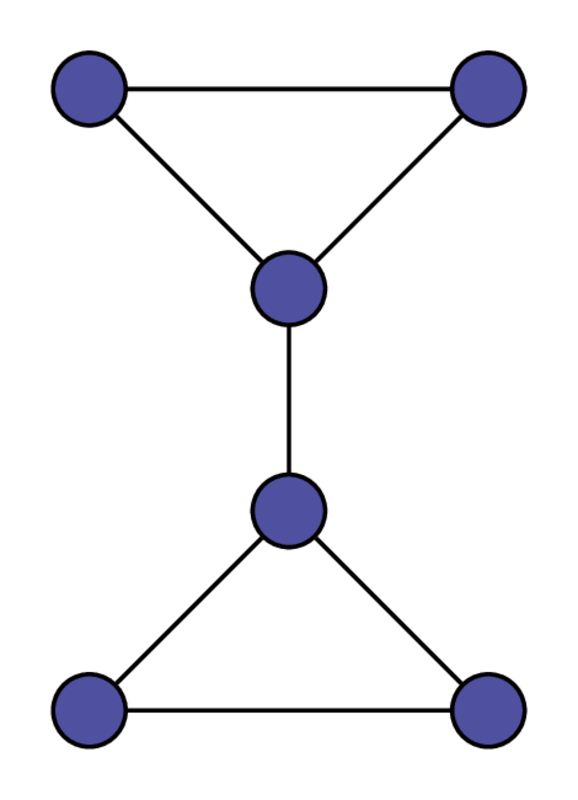
\includegraphics[height=8cm,width=.3\textwidth]{exercise7/diagrams/d1.png}\end{center}

\end{enumerate}
